\documentclass{article} \usepackage[utf8]{inputenc}
\usepackage{amsmath, amssymb, systeme, mathtools, lmodern, float, graphicx}
\usepackage[most]{tcolorbox}
\usepackage[scale=.95,type1]{cabin}
\usepackage[framemethod=tikz]{mdframed}

\usepackage[legalpaper,margin=1in]{geometry}

\setlength{\parindent}{10pt}
\setlength{\parskip}{1em}
\renewcommand{\baselinestretch}{1.2}

\title{Chapter 7: Eigenvalues and Eigenvectors}
\date{}

\makeatletter
\renewcommand*\env@matrix[1][*\c@MaxMatrixCols c]{%
  \hskip -\arraycolsep
  \let\@ifnextchar\new@ifnextchar
  \array{#1}}
\makeatother

\newcommand\y{\cellcolor{blue!10}}

\usepackage{tabularray}
\SetTblrInner{colsep=5pt,rowsep=1pt}

\newcommand\x{\times}
\newcommand\xor{\oplus}

\newcommand\R{\mathbb{R}}

\DeclarePairedDelimiter\abs{\lvert}{\rvert}%
\DeclarePairedDelimiter\norm{\lVert}{\rVert}%

% Swap the definition of \abs* and \norm*, so that \abs
% and \norm resizes the size of the brackets, and the 
% starred version does not.
\makeatletter
\let\oldabs\abs
\def\abs{\@ifstar{\oldabs}{\oldabs*}}
%
\let\oldnorm\norm
\def\norm{\@ifstar{\oldnorm}{\oldnorm*}}
\makeatother

\newcommand*{\Value}{\frac{1}{2}x^2}%

\newcommand\ddfrac[2]{\frac{\displaystyle #1}{\displaystyle #2}}


\newcounter{Def}[section]
\newenvironment{Def}[1][]{%
  \ifstrempty{#1}%
  {\mdfsetup{%
    frametitle={%
      \tikz[baseline=(current bounding box.east),outer sep=0pt]
      \node[line width=1pt,anchor=east,rectangle,draw=blue!20,fill=white]
    {\strut \color{black}{Definition}~};}}
  }%
  {\mdfsetup{%
    frametitle={%
      \tikz[baseline=(current bounding box.east),outer sep=0pt]
      \node[line width=1pt,anchor=east,rectangle,draw=blue!20,fill=white]
    {\strut \color{black}{Definition}~:~\color{blue4}{#1}};}}%
  }%
  \mdfsetup{innertopmargin=2pt,linecolor=blue!20,%
            linewidth=1pt,topline=true,%
            frametitleaboveskip=\dimexpr-\ht\strutbox\relax,}
  \begin{mdframed}[]\relax%
  }{\end{mdframed}}

\begin{document}

    \begin{Def}[    Type constructors]    
    Used only in type level, type signatures, and typeclass declarations and instances. Types are
    static and resolve at compile time.
    \end{Def}
    
    \begin{Def}[Data constructors]
    Data constructors construct the values at term level, values you can interact with
    at runtime.
        
    \end{Def}

    Kinds are types of types, 1 level up, and is represented with *.

    \section{Type and Data}

    Types are static and resolve at compile time. Data are what we're working at runtime.

    Compile time is when the program is getting compiled by GHC before execution. Runtime
    is the actual execution.

    \section{Data constructor arities }
    \textit{Arity} refers to the number of arguments of a function or constructor takes. \textit{Nullary}
    is a function taking no arguments (null - ary). \textit{Unary} refers to data constructors that
    take one argument. \textit{Products} are those take more than one arguments.
    
    \begin{Def}[Algebraic]
        Algebraic datatypes are algebraic since the patterns of argument structures using 2 
        basic operations: \textit{sum} and \textit{product}.
    \end{Def}

    \begin{Def}[Cardinality]
        The cardinality of a datatype is the number of possible values it defines.
    \end{Def}

    The value will be constructed at runtime from the argument we applied it to.

    \subsection*{newtype}
    A newtype has no runtime overhead, as it reuses the representation of the type it contains.
    
    \includegraphics*[width = 7cm]{pragma.png}

    With this pragma, no need to declare again.

    \section{Record syntax}
    Records are product types with additional syntax to provide convinient accessors to fields
    within the record.

    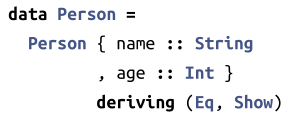
\includegraphics[width = 5cm]{recordsyntax.png}

    They are just functions that take a member of the product. (age papu...)

    And records are just syntax to create field references.

    \subsection*{Distributive property}
    Just like $a . (b + c) = a . b + a . c$, that's the normal form.

    \subsection*{Constructing and deconstructing values (duality)}

    \begin{Def}[Type synonyms]
    Try to avoid using \textit{type synonyms} with unstructured data like text or binary. It's best used
    when you want something \textit{lighter weight} than newtypes but also want the type signatures
    to be more explicit.
    \end{Def}

    The total values is the product of the number of inhabitants.

    \subsubsection*{Deconstructing values}
    Recall that \textit{catamorphism} are means of deconstructing data, breaking down
    any datatype. If the spine of a list
    is the structure of it, then fold can reduce the structure.

    Unpacking or deconstructing the contents of a product type.

    \subsection*{Function type is exponential}

    The number of inhabitants of $a -> b$ is $b^a$.

    \section{Higher-kinded datatypes}
    Recall that kinds are types of type constructors. Kinds are not type until they are fully
    applied.

    Lists are polymorphic until the type's argument has been fully applied:

    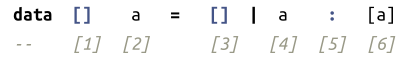
\includegraphics[width = 6cm]{list.png}

    "[]" : Type constructor for list (special syntax), take "a" as argument. The colon is
    an infix data constructor, it is the product of a and [a].

    \subsection*{Infix type and data constructors}
    An operator that has non-alphanumeric name is \textbf{infix} by default. Any operator that starts
    with (:) must be an infix type or data constructor. All infix data constructors start with
    a colon.
    The type constructor of functions, ($\to$), is the only exception. (:: is type assertions)

    \begin{Def}[The difference]
        Type constructors are functions one level up, structuring things that cannot exist
        at runtime - it's purely static and describes the structure of your types.
    \end{Def}

    \section{Binary Tree} 
    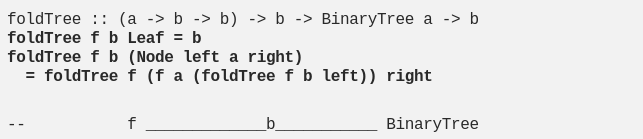
\includegraphics[width = 12cm]{foldrTree.png}

    This is, roughly, what is being generated by the automatic \textit{deriving Foldable}.

    Magic spell: \{\-\# LANGUAGE DeriveFoldable \#\-\}, and then foldTree = foldr.

    The above is a \textit{sequential} fold, which first folds over the left part, then over the middle
    element, then over the right.

    \section{Hutton's Razor}
    













\end{document}
